\chapter{Novel Datasets for Transfer Learning}

\begin{remark}{Outline}

This chapter ...

\vspace{5mm}
\textit{This chapter is based on the publication \citet{sabatelli2021advances}.}
\label{ch:minerva_paper}


\end{remark}


\section{Challenges of Modern Computer Vision}
\label{sec:cv_challenges}

If it is true that the results presented in the previous chapter show that it is possible to successfully transfer pre-trained convolutional neural networks to non natural image datasets, it is equally true that some limitations might still need to be addressed. One above all, is the need of fine-tuning the networks instead of simply using them as feature extractors. As demonstrated by the experiments performed on the third classification problem of the Rijksmuseum dataset, it is clear that pre-trained models might only learn features that are relevant for their respective source task $\mathcal{T}_S$ (ImageNet), which therefore might result into unsatisfying performance when an off the shelf training strategy is used. While this is a result that does not come as a surprise, as it would be unreasonable to expect pre-trained networks to act as universal feature extractors, this limitation can still have some important practical implications, since it can prevent the deployment of computer vision systems outside the domain of natural images. As a very practical example let us consider the first image presented in Fig. \ref{fig:fails} and the computer vision task of object detection. We tackle this task with an object detector that is pre-trained on natural images only and that therefore, has never seen any images coming from a domain other than the source domain $\mathcal{D}_S$. From the performance of the model it is clear that only one out of the two predictions made by the network is appropriate, as it fails in detecting the musical instrument depicted in the image by wrongly classifying it as a `frisbee". While certainly reasonable and fully justifiable, this kind of performance is the result of some limitations that currently characterize modern Computer Vision (CV) which we summarize as follows:

\begin{itemize}
	\item \textcolor{RoyalBlue}{Photorealism and Data Scarcity:} it is well known that modern CV strongly gravitates towards photorealistic material, since most of the datasets that are used in the field are representative of digitized, or born-digital, versions of photographs. Nevertheless, datasets like MNIST, CIFAR-10/100 and the already mentioned ImageNet play a crucial role in today's rapid development of the field, as they are constantly used as benchmarks by the community. While certainly suitable for defining different challenging CV tasks, it is worth noting however, that these datasets are also only partially representative of the physical world, as they do not actively attempt to distort the reality they depict. Unfortunately, datasets going beyond the photorealistic domain are either much rarer, or are simply not as popular as their photorealistic counterparts, a limitation that results into pre-trained models that fail in performing well when used outside from the natural world (see again first image of Fig. \ref{fig:fails}).  

	\item \textcolor{RoyalBlue}{Modern Training Classes:} the performance depicted in the first image of Fig. \ref{fig:fails} can largely be attributed to the fact that the model used for detecting the objects in the image has never been explicitly trained on images of musical instruments. As a result its predictions can only tend to be representative of the classes that have governed the training process. While this is a behavior that has only to be expected, it can still serve as a surrogate for highlighting a crucial limitation of modern object detection datasets: datasets are not as diversified and heterogeneous as one might expect. As an example let us consider the popular Pascal-Voc \cite{everingham2010pascal} and MS-COCO \cite{lin2014microsoft} datasets. The first one tackles the detection of 20 classes, out of which more than a third constitute different kinds of transportation systems, such as `trains", `boats",`motorcycles" and `cars". The latter, albeit more complex, mostly represents objects that are representative of the highly technological world we currently live in, with classes such as `microwave", `laptop" and `remote control". In practice this results into models that gravitate towards detecting objects in an image which are modern, a behavior that hurts not-technological classes such as the `person" one which should be detected in the second image of Fig. \ref{fig:fails}.     

	\item \textcolor{RoyalBlue}{Model Robustness:} the aforementioned limitation also results into models that learn features that are hardly general enough for successfully tackling different representations of the same class. As an example let us consider the last image of Fig. \ref{fig:fails}: we can clearly see that a model pre-trained on MS-COCO successfully detects the persons represented in the paintings only as long as their pose corresponds to a pose that can easily be found in the images depicting persons in photorealistic datasets. As soon as a person is depicted in a pose that is different from the one that usually characterizes a person in a photorealistic dataset (sitting or standing), then a pre-trained network mistakenly detects it as an animal.   
\end{itemize}

\begin{figure}[ht!]
\centering
  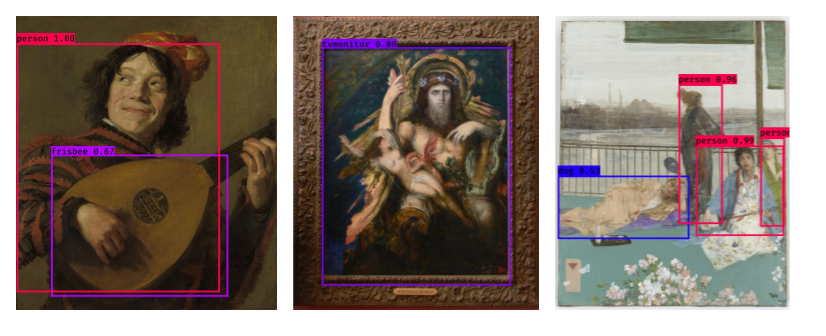
\includegraphics[width=\linewidth]{./Images/Chapter05/fails}
  \caption{}
  \label{fig:fails}
\end{figure}

In this chapter we take inspiration from these limitations and use them as a surrogate for introducing novel datasets that can be used as a benchmark for CV researchers. The purpose of such datasets is twofold: on the one hand they represent, at least in part, a solution to the aforementioned issues that currently characterize CV, while on the other hand, they allow us to continue studying the transfer learning properties of convolutional neural networks which we started in the previous chapter.  

\section{The MINERVA Dataset}
\label{sec:minerva_dataset}

We now introduce MINERVA, a novel annotated dataset that can be used for object detection. More specifically, the main task that we present is that of the detection of musical instruments in non-photorealistic, unrestricted image collections from the artistic domain. We start by providing some background information about the field of music iconography which allows us to motivate why being able to identify musical instruments is not only a challenging CV task but is also of high practical interest. We then describe how the images of MINERVA have been first collected and then annotated. We end this section by quantitatively characterizing the dataset from a machine learning perspective.    

\subsection{Music Iconography}


\subsection{Data Collection}
The images constituting MINERVA come from three different data sources which allow the dataset to be highly varied and unrestricted. In fact its images cover a large range of periods, genres and materials and are both of photorealistic and not-photorealistic nature as visually represented in Fig. \ref{fig:minerva_dataset}. The three data sources are the following:
\begin{itemize}
	\item RIDIM: which stays for \textit{Repertoire International d'Iconographie Musicale} is an international digital inventory for musical iconography that functions as a reference image database. Developed and curated by \citet{green2013ridim} it has been designed to facilitate the discovery of music-related artworks. Among the three different considered data sources, the images coming from the RIDIM collection are the ones of highest quality in terms of resolution.
	\item RMFAB/RMAH: which stays for \textit{Royal Museums of Fine Arts of Belgium} and \textit{Royal Museums of Art and History}. These images come from a larger pool of digitized images which have been manually selected on the basis whether they included depictions of musical instruments or not. Among the different data sources, the amount of images coming from RMFAB/RMAH within MINERVA is is the lowest when compared to the other two data sources. These images are of midrange resolution.
	\item Flickr: is a well known image hosting service from which we downloaded a large dataset of images depicting musical instruments in the visual arts pre-dating 1800. Most of the images present within MINERVA come from Flickr, although their resolution is not always on par with the previous two data sources.  
\end{itemize}

Once all these images have been collected we have started the labeling process.

\subsection{Annotation Process}

We manually annotated almost $10000$ instruments by using the conventional method of rectangular bounding boxes. To this end we have used the open-source \texttt{Cytomine} software \cite{maree2016collaborative}, a rich web environment that allows highly collaborative analysis of multi-gigapixel imaging data. Originally developed for facilitating the task of image annotation in biomedical informatics, \texttt{Cytomine} has already been widely used for the annotation and creation of several datasets \cite{mormont2018comparison}. However, it is worth noting that its use within the present study is among the very first ones which uses the software outside the context of large-scale biomaging data. Regarding the labeling process itself, all the individual instruments within MINERVA have been unambiguously identified and labeled by using their MIMO codes. The MIMO (Musical Instrument Museums Online) initiative is an international consortium, well known for its online database of musical instruments, aggregating data and metadata from multiple heritage institutions \cite{dolan2017mimo}. An important contribution of \citet{dolan2017mimo} is the development of a uniform metadata documentation standard for the field, including a multilingual vocabulary that can be used for identifying musical instruments in an interoperable manner. We have followed this metadata standard and manually labeled the previously collected images within \texttt{Cytomine} as visually represented in Fig. \ref{}.

\subsection{Versions and Splits}

MINERVA comes in four, different, increasingly complex, versions: \texttt{Minerva-0} which is arguably the easiest version of the dataset where the target task $\mathcal{T}_T$ simply consists in detecting whether a musical instrument is present within an image or not. We therefore do not yet consider the task of predicting the class of the detected instrument. The second version of the dataset is \texttt{Minerva-Hypernym} where the goal is that of detecting all the images present within \texttt{Minerva-0} and classify them according to their hypernym categories. All instruments present within MINERVA correspond to $5$ different hypernyms which define them as: `stringed instruments", `wind instruments", `percussion instruments", `keyboard instruments" and `electronic instruments'. The last two versions of MINERVA are \texttt{Minerva-5} and \texttt{Minerva-10} where the goal is to detect and classify the instruments depicted in the images according to the top 5 or top 10 most occurring classes. These classes are: `Lute", `Harp", `Violin", `Trumpet", `Shawn", `Bagpipe", `Organ", `Horn", `Rebec" and `Lyre". Naturally, in \texttt{Minerva-5} we only consider the first $5$ of such classes, whereas in \texttt{Minerva-10} we consider all $10$ of them. Each version of the dataset comes with its own training, validation and testing splits, where we offer the guarantee that at least one of the instrument classes in the task is represented in each of the splits. Additionally, the splits are stratified so that the class distribution is approximately the same in each split. The number of images per split in each version is summarized in Table \ref{table:minerva_splits} where $N_t$ corresponds to the amount of images present within the split, whereas $I_t$ denotes the number of total instruments. The hypernym version of the dataset is not reported as it shares the same images and splits as \texttt{Minerva-0} (they both contain all instruments), however a distribution of the hypernym classes within \texttt{Minerva-Hypernym} is reported in Fig. \ref{fig:hypernym_distribution}. All splits have been created with the \texttt{scikit-learn} software \cite{pedregosa2011scikit} by using $50\%$ of the images for training, and the remaining $50\%$ for validation and testing ($25\%$ respectively). 

\begin{table}
\begin{tabular}{l|rr|rr|rr} \hline
	$\mathcal{T}_T$ &  \multicolumn{2}{c}{training-set} & \multicolumn{2}{|c|}{validation-set} & \multicolumn{2}{c}{testing-set}\\
& $N_t$ & $I_t$ & $N_t$ & $I_t$ & $N_t$ & $I_t$ \\\hline \hline
\texttt{Minerva-0} & 1857 & 4243 & 1137 & 2288 & 1182 & 2102 \\
\texttt{Minerva-5} & 952 & 1589 & 540 & 852 & 721 & 1173\\
\texttt{Minerva-10} & 1227 & 2147  & 680 & 1127 & 897 & 1506 \\
\hline

\end{tabular}

\caption{An overview reporting how many images $N_t$ and instruments $I_t$ are present within the splits of the \texttt{Minerva-0, Minerva-5} and \texttt{Minerva-10} versions of the MINERVA dataset.}
\label{table:minerva_splits}
\end{table}

\begin{figure}[htb!]
	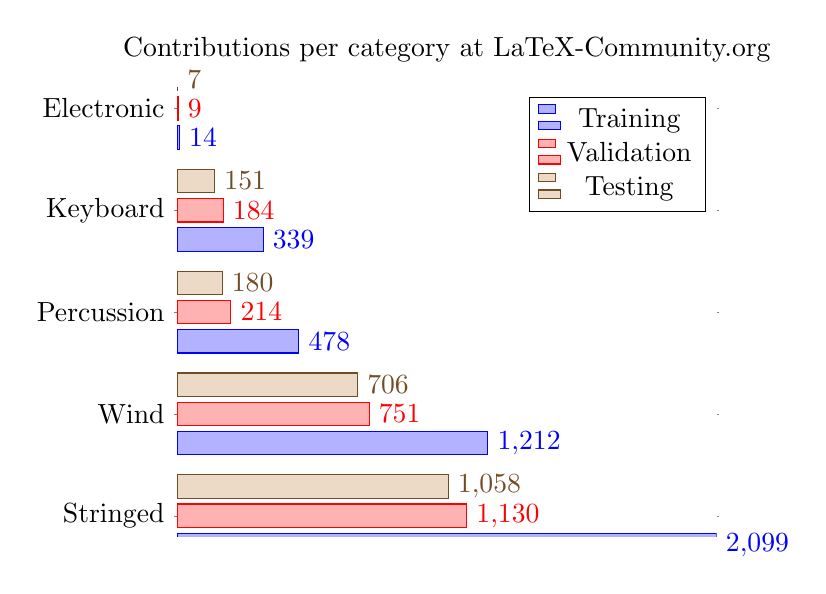
\begin{tikzpicture}
  \begin{axis}[title  = Contributions per category
                          at LaTeX-Community.org,
    xbar,
    bar width=.3cm,
    y axis line style = { opacity = 0 },
    axis x line       = none,
    tickwidth         = 1pt,
    enlarge y limits  = 0.05,
    enlarge x limits  = 0.001,
    symbolic y coords = {Stringed, Wind, Percussion,Keyboard, Electronic},
    nodes near coords,
  ]
\addplot coordinates {(2099,Stringed) (1212,Wind) (478,Percussion) (339,Keyboard) (14,Electronic)};
\addplot coordinates {(1130,Stringed) (751,Wind) (214,Percussion) (184,Keyboard) (9,Electronic)};
\addplot coordinates {(1058,Stringed) (706,Wind) (180,Percussion) (151,Keyboard) (7,Electronic)};
\legend{Training,Validation,Testing}

\end{axis}
\end{tikzpicture}

\iffalse
\end{axis}
\end{tikzpicture}
\fi

	\caption{A visual representation of the distribution of the hypernym classes that are present within \texttt{Minerva-0} and that define the \texttt{Minerva-Hypernym} benchmark.}
	\label{fig:hypernym_distribution}
\end{figure}


\section{Benchmarking}
\label{sec:benchmarking}

While MINERVA has been created with the primary intention of serving as a novel dataset for object detection, it can nevertheless still be used for testing the classification performance of convolutional neural networks as well. Although this task is certainly easier than the one of object detection, it is still of high interest as it provides a novel benchmark for further characterizing the transfer learning properties of neural networks that we started studying in the previous chapter. Therefore, we hereafter report results both for \textcolor{RoyalBlue}{classification} experiments as for \textcolor{RoyalBlue}{object detection} experiments. In the first section we consider the target task $\mathcal{T}_T$ of classifying the bounding boxes that have been annotated in MINERVA as standalone images, while in the second section we aim at both detecting and classifying the content of the potentially detected bounding boxes. We hereafter describe the experimental protocol used for both sets of experiments into detail.

\subsection{Classification}
The experimental setup used for the classification experiments largely builds on top of the study that we presented in Chapter \ref{ch:tl_natural_to_non_natural}. We continue to explore whether popular neural architectures, that have obtained state of the art results on the ImageNet benchmark, are able to perform equally well when they are trained on datasets of non natural images. To this end, we again consider the well known VGG19 \cite{simonyan2014very}, InceptionV3 \cite{szegedy2016rethinking} and ResNet50 \cite{xie2017aggregated} neural architectures. As done in the previous chapter we keep investigating the effect that different weight initialization strategies have on the final performance of the networks, with the goal of further characterizing the potential benefits that can come from adopting transfer learning. Specifically, we train the three considered neural architectures by following three different initalization strategies: `random" which simply initializes the model's parameters after following a initalization strategy, `ImageNet" which instead uses the weights that have been obtained after training the networks on the ImageNet source task $\mathcal{T}_S$, and `RijksNet" which are the models we trained both on the ImageNet dataset and on the Rijksmuseum collection, and that were also used for the final experiments of the previous chapter. For this study we only fine tune the networks, while we do not explore their performance when they are used as off the shelf feature extractors. We train all networks with the Adam optimizer \cite{kingma2014adam} and by using an initial learning rate of $0.001$. As already done for the previous study, we again controlled the training process by using early stopping and by interrupting the training regime as soon as the validation loss did not decrease for five epochs in a row. Naturally, all networks minimize the categorical crossentropy loss function.

\subsection{Object Detection}

\begin{aligned}
& \lambda_\text{coord} \sum_{i=1}^{S \times S} \sum_{j=1}^B \mathbb{1}_{i,j}^\text{obj} \left( (x_i - \hat{x}_{i,j})^2 + (y_i - \hat{y}_{i,j})^2 + (\sqrt{w_i} - \sqrt{\hat{w}_{i,j}})^2 + (\sqrt{h_i} - \sqrt{\hat{h}_{i,j}})^2\right)\\\\
& + \lambda_\text{obj} \sum_{i=1}^{S \times S} \sum_{j=1}^B \mathbb{1}_{i,j}^\text{obj} (c_{i,j} - \hat{c}_{i,j})^2 + \lambda_\text{noobj} \sum_{i=1}^{S \times S} \sum_{j=1}^B (1-\mathbb{1}_{i,j}^\text{obj}) \hat{c}_{i,j}^2  \\\\
& + \lambda_\text{classes} \sum_{i=1}^{S \times S} \mathbb{1}_i^\text{obj} \sum_{c=1}^C (p_{i,c} - \hat{p}_{i,c})^2 
\end{aligned}


where $\hat{p}{i,c}$, $\hat{x}{i,j}$, $\hat{y}{i,j}$, $\hat{w}{i,j}$, $\hat{h}{i,j}$ and $\hat{c}{i,j}$ are the network outputs.




\section{Results}
\label{sec:results}

\subsection{Quantitative Analysis}
\paragraph{Classification}


\begin{table}
    \caption{An overview reporting how many images $N_t$ and instruments $I_t$ are present within the splits of the \texttt{Minerva-0, Minerva-5} and \texttt{Minerva-10} versions of the MINERVA dataset.}
\resizebox{\columnwidth}{!}{%
	\begin{tabular}{l|cc|cc|cc} \hline
	$\mathcal{T}_T$ &  \multicolumn{2}{c}{ResNet50} & \multicolumn{2}{|c|}{InceptionV3} & \multicolumn{2}{c}{VGG19}\\
			& Accuracy ($\%$) & F1 & Accuracy ($\%$) & F1 & Accuracy $(\%)$ & F1 \\\hline \hline
	\texttt{Minerva-Hypernym} & 72.26 & 52.66 & \cellcolor{green!25}{75.80} & \cellcolor{green!25}{57.03} & 66.41 & 40.35 \\
	\texttt{Minerva-5} & 68.71  & 64.10 & \cellcolor{green!25}{73.66} & \cellcolor{green!25}{70.29} & 48.33 & 33.92\\
	\texttt{Minerva-10} & 52.85 & 41.55  & \cellcolor{green!25}{55.51} & \cellcolor{green!25}{44.77} & 37.52 & 15.22 \\
\hline
\end{tabular}
%
}
\label{table:minerva_splits}
\end{table}


\iffalse
\begin{figure}[htb!]
	%The matrix in numbers
%Horizontal target class
%Vertical output class
\def\myConfMat{{
{0.01,  30,  60,  10,  20,  30,  40,  50,  60,  60},  %row 1
{0.01,  30,  60,  10,  20,  30,  40,  50,  60,  60},  %row 2
{0.01,  30,  60,  10,  20,  30,  40,  50,  60,  60},  %row 3
{0.01,  30,  60,  10,  20,  30,  40,  50,  60,  20},  %row 4
{0.01,  30,  60,  10,  20,  30,  40,  50,  60,  20},  %row 5
{0.01,  30,  60,  10,  20,  30,  40,  50,  60,  20},  %row 6
{0.01,  30,  60,  10,  20,  30,  40,  50,  60,  20},  %row 7
{0.01,  30,  60,  10,  20,  30,  40,  5,  60,  20},  %row 8
{0.01,  30,  60,  10,  20,  30,  40,  50,  60, 20},  %row 9
{0.01,  30,  60,  10,  20,  30,  40,  50,  60,  20},  %row 10
}}

\def\classNames{{"A","B","C","D","E","F","G","H","I","J"}} %class names. Adapt at will

\def\numClasses{10} %number of classes. Could be automatic, but you can change it for tests.

\def\myScale{1.5} % 1.5 is a good scale. Values under 1 may need smaller fonts!
\begin{tikzpicture}[
    scale = \myScale,
    font={\scriptsize}, %for smaller scales, even \tiny may be useful
    ]

\tikzset{vertical label/.style={rotate=90,anchor=east}}   % usable styles for below
\tikzset{diagonal label/.style={rotate=45,anchor=north east}}

\foreach \y in {1,...,\numClasses} %loop vertical starting on top
{
    % Add class name on the left
    \node [anchor=east] at (0.4,-\y) {\pgfmathparse{\classNames[\y-1]}\pgfmathresult}; 
    
    \foreach \x in {1,...,\numClasses}  %loop horizontal starting on left
    {
%---- Start of automatic calculation of totSamples for the column ------------   
    \def\totSamples{0}
    \foreach \ll in {1,...,\numClasses}
    {
        \pgfmathparse{\myConfMat[\ll-1][\x-1]}   %fetch next element
        \xdef\totSamples{\totSamples+\pgfmathresult} %accumulate it with previous sum
        %must use \xdef fro global effect otherwise lost in foreach loop!
    }
    \pgfmathparse{\totSamples} \xdef\totSamples{\pgfmathresult}  % put the final sum in variable
%---- End of automatic calculation of totSamples ----------------
    
    \begin{scope}[shift={(\x,-\y)}]
        \def\mVal{\myConfMat[\y-1][\x-1]} % The value at index y,x (-1 because of zero indexing)
        \pgfmathtruncatemacro{\r}{\mVal}   %
        \pgfmathtruncatemacro{\p}{round(\r/\totSamples*100)}
        \coordinate (C) at (0,0);
        \ifthenelse{\p<50}{\def\txtcol{black}}{\def\txtcol{white}} %decide text color for contrast
        \node[
            draw,                 %draw lines
            text=\txtcol,         %text color (automatic for better contrast)
            align=center,         %align text inside cells (also for wrapping)
            fill=black!\p,        %intensity of fill (can change base color)
            minimum size=\myScale*10mm,    %cell size to fit the scale and integer dimensions (in cm)
            inner sep=0,          %remove all inner gaps to save space in small scales
            ] (C) {\r\\\p\%};     %text to put in cell (adapt at will)
        %Now if last vertical class add its label at the bottom
        \ifthenelse{\y=\numClasses}{
        \node [] at ($(C)-(0,0.75)$) % can use vertical or diagonal label as option
        {\pgfmathparse{\classNames[\x-1]}\pgfmathresult};}{}
    \end{scope}
    }
}
%Now add x and y labels on suitable coordinates
\coordinate (yaxis) at (-0.3,0.5-\numClasses/2);  %must adapt if class labels are wider!
\coordinate (xaxis) at (0.5+\numClasses/2, -\numClasses-1.25); %id. for non horizontal labels!
\node [vertical label] at (yaxis) {Output Class};
\node []               at (xaxis) {Target Class};
\end{tikzpicture}
}

	\caption
	\label{fig:hypernym_distribution}
\end{figure}
\fi




\paragraph{Object Detection}



\begin{figure}[htb!]
	\scalebox{0.8}{\begin{minipage}{.5\textwidth}
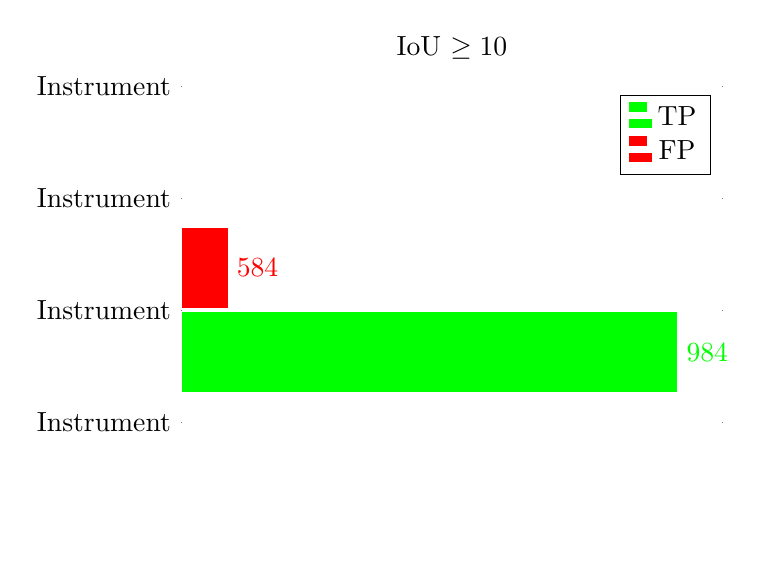
\begin{tikzpicture}
  \begin{axis}[title  = IoU $\geq 10$,
    xbar,
    bar width=1cm,
    y axis line style = { opacity = 0 },
    axis x line       = none,
    tickwidth         = 0.5pt,
    symbolic y coords = {Instrument},
    nodes near coords,
  ]
  \addplot [color=green,fill ] coordinates {(984,Instrument)};
  \addplot [color=red,fill] coordinates {(584,Instrument)};
\legend{TP,FP}
\end{axis}
\end{tikzpicture}
 \end{minipage}
 \hspace{3cm}
\begin{minipage}{.5\textwidth}
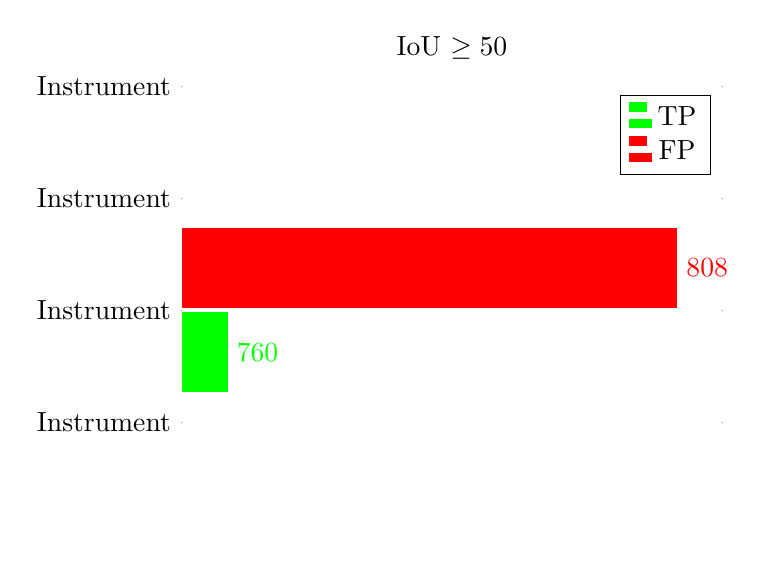
\begin{tikzpicture}
  \begin{axis}[title  = IoU $\geq 50$,
    xbar,
    bar width=1cm,
    y axis line style = { opacity = 0 },
    axis x line       = none,
    tickwidth         = 0.5pt,
    symbolic y coords = {Instrument},
    nodes near coords,
  ]
  \addplot [color=green,fill] coordinates {(760,Instrument)};
  \addplot [color=red,fill] coordinates {(808,Instrument)};
\legend{TP,FP}

\end{axis}
\end{tikzpicture}
 \end{minipage}
 

}
	\caption{}
	\label{fig:detection_experiment_1}
\end{figure}


\begin{figure}[htb!]
	\scalebox{0.8}{\begin{minipage}{.5\textwidth}
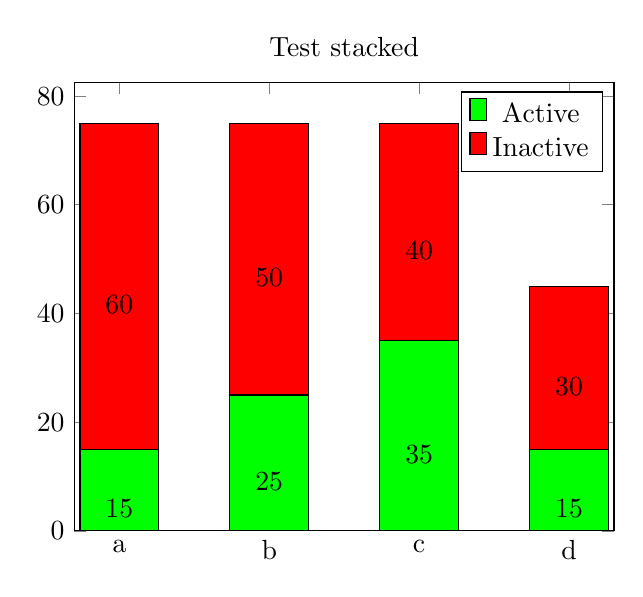
\begin{tikzpicture}
  \begin{axis}[
    title={Test stacked},
    ybar stacked, ymin=0,  
    bar width=10mm,
    symbolic x coords={a,b,c,d},
    xtick=data,
    nodes near coords, 
    nodes near coords align={anchor=north},%Move values in bar
    every node near coord/.style={
    },
  ]
  %Active
  \addplot [fill=green] coordinates {
({a},15)
({b},25)
({c},35)
({d},15)};
  %Inactive
  \addplot [fill=red] coordinates {
({a},60)
({b},50)
({c},40)
({d},30)};
  \legend{Active,Inactive}
  \end{axis}
 \end{tikzpicture}
 \end{minipage}
 \hspace{2.5cm}
\begin{minipage}{.5\textwidth}
 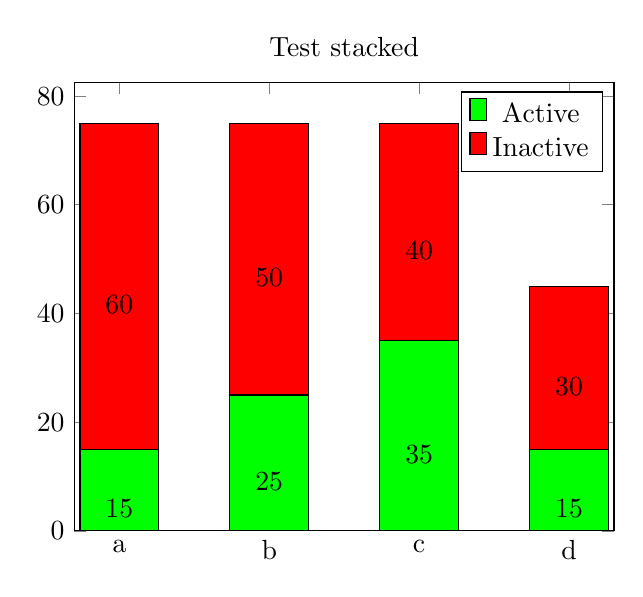
\begin{tikzpicture}
  \begin{axis}[
    title={Test stacked},
    ybar stacked, ymin=0,  
    bar width=10mm,
    symbolic x coords={a,b,c,d},
    xtick=data,
    nodes near coords, 
    nodes near coords align={anchor=north},%Move values in bar
    every node near coord/.style={
    },
  ]
  %Active
  \addplot [fill=green] coordinates {
({a},15)
({b},25)
({c},35)
({d},15)};
  %Inactive
  \addplot [fill=red] coordinates {
({a},60)
({b},50)
({c},40)
({d},30)};
  \legend{Active,Inactive}
  \end{axis}
 \end{tikzpicture}
 \end{minipage}

}
	\caption{}
	\label{fig:detection_experiment_2}
\end{figure}



\begin{figure}[htb!]
	\scalebox{0.8}{\begin{minipage}{.5\textwidth}
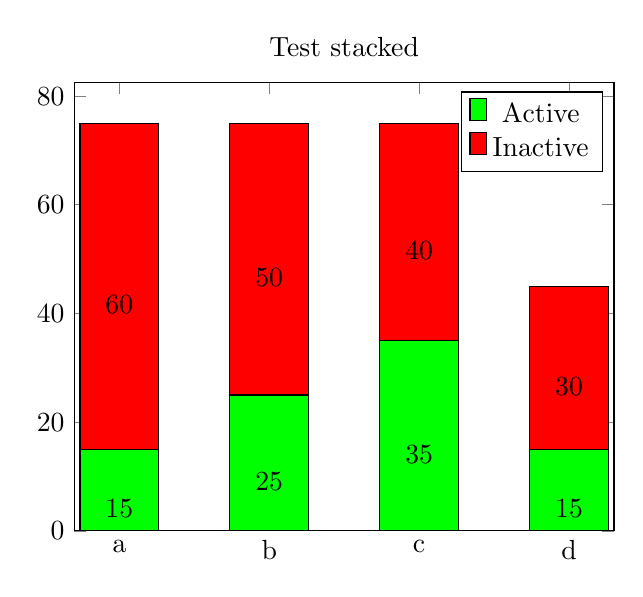
\begin{tikzpicture}
  \begin{axis}[
    title={Test stacked},
    ybar stacked, ymin=0,  
    bar width=10mm,
    symbolic x coords={a,b,c,d},
    xtick=data,
    nodes near coords, 
    nodes near coords align={anchor=north},%Move values in bar
    every node near coord/.style={
    },
  ]
  %Active
  \addplot [fill=green] coordinates {
({a},15)
({b},25)
({c},35)
({d},15)};
  %Inactive
  \addplot [fill=red] coordinates {
({a},60)
({b},50)
({c},40)
({d},30)};
  \legend{Active,Inactive}
  \end{axis}
 \end{tikzpicture}
 \end{minipage}
 \hspace{2.5cm}
\begin{minipage}{.5\textwidth}
 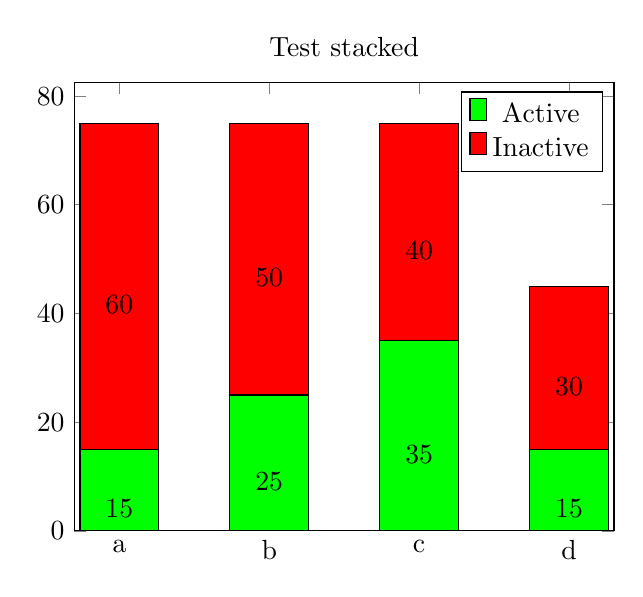
\begin{tikzpicture}
  \begin{axis}[
    title={Test stacked},
    ybar stacked, ymin=0,  
    bar width=10mm,
    symbolic x coords={a,b,c,d},
    xtick=data,
    nodes near coords, 
    nodes near coords align={anchor=north},%Move values in bar
    every node near coord/.style={
    },
  ]
  %Active
  \addplot [fill=green] coordinates {
({a},15)
({b},25)
({c},35)
({d},15)};
  %Inactive
  \addplot [fill=red] coordinates {
({a},60)
({b},50)
({c},40)
({d},30)};
  \legend{Active,Inactive}
  \end{axis}
 \end{tikzpicture}
 \end{minipage}

}
	\caption{}
	\label{fig:detection_experiment_3}
\end{figure}


\begin{figure}[htb!]
	\scalebox{0.8}{\begin{minipage}{.5\textwidth}
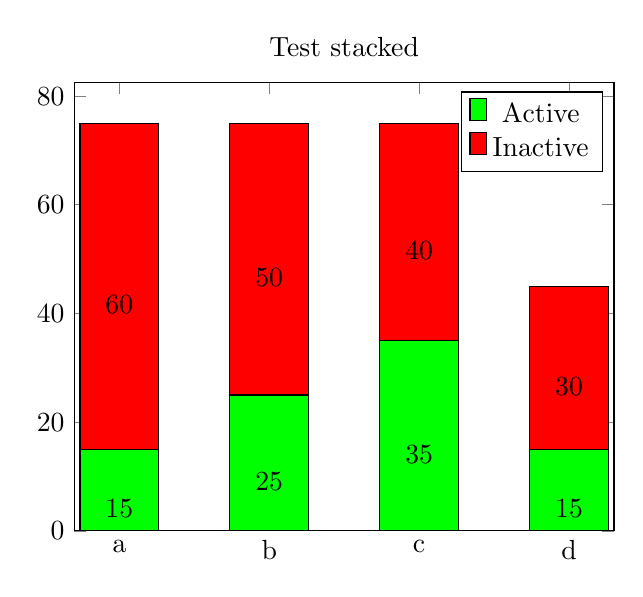
\begin{tikzpicture}
  \begin{axis}[
    title={Test stacked},
    ybar stacked, ymin=0,  
    bar width=10mm,
    symbolic x coords={a,b,c,d},
    xtick=data,
    nodes near coords, 
    nodes near coords align={anchor=north},%Move values in bar
    every node near coord/.style={
    },
  ]
  %Active
  \addplot [fill=green] coordinates {
({a},15)
({b},25)
({c},35)
({d},15)};
  %Inactive
  \addplot [fill=red] coordinates {
({a},60)
({b},50)
({c},40)
({d},30)};
  \legend{Active,Inactive}
  \end{axis}
 \end{tikzpicture}
 \end{minipage}
 \hspace{2.5cm}
\begin{minipage}{.5\textwidth}
 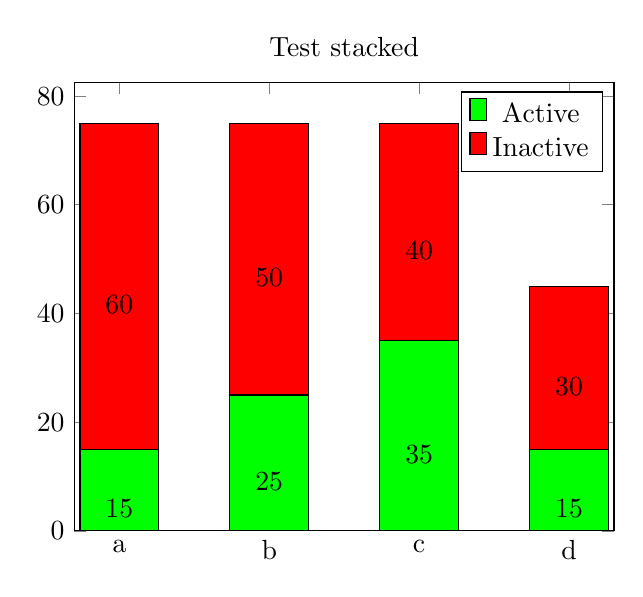
\begin{tikzpicture}
  \begin{axis}[
    title={Test stacked},
    ybar stacked, ymin=0,  
    bar width=10mm,
    symbolic x coords={a,b,c,d},
    xtick=data,
    nodes near coords, 
    nodes near coords align={anchor=north},%Move values in bar
    every node near coord/.style={
    },
  ]
  %Active
  \addplot [fill=green] coordinates {
({a},15)
({b},25)
({c},35)
({d},15)};
  %Inactive
  \addplot [fill=red] coordinates {
({a},60)
({b},50)
({c},40)
({d},30)};
  \legend{Active,Inactive}
  \end{axis}
 \end{tikzpicture}
 \end{minipage}

}
	\caption{}
	\label{fig:detection_experiment_4}
\end{figure}




\subsection{Qualitative Analysis}
\paragraph{True vs False Positives}
\paragraph{Saliency Maps}


\section{Discussion and Critical Analysis}
\label{sec:discussion}


\section{Future Work: towards more benchmarks}
\label{sec:future_work}
